
% !TEX encoding = UTF-8 Unicode


\documentclass{beamer}

\usetheme{Madrid}
\usepackage{graphicx}
\usepackage{epstopdf}
\DeclareGraphicsExtensions{.eps}
\usepackage{url}
\usepackage{multicol}% http://ctan.org/pkg/multicols





  \usepackage{cite}




\usepackage[utf8x]{inputenc} 


\usepackage{array}
\newcolumntype{L}[1]{>{\raggedright\let\newline\\\arraybackslash\hspace{0pt}}m{#1}}
\newcolumntype{C}[1]{>{\centering\let\newline\\\arraybackslash\hspace{0pt}}m{#1}}
\newcolumntype{R}[1]{>{\raggedleft\let\newline\\\arraybackslash\hspace{0pt}}m{#1}}

\usepackage{float}

\usepackage{siunitx}
\usepackage{amsmath}
\usepackage{amsfonts}
\usepackage{amssymb}

\usepackage[utf8]{inputenc}

\title{Introdução ao NAS Parallel Benchmarks}

\subtitle{Performance Relativa de Kernels Sequenciais, em ambiente de Memória Partilhada e ambiente de Memória Distribuída}
% A subtitle is optional and this may be deleted

           
\author{ Filipe Costa Oliveira}


\institute[Universidade of Minho] % (optional, but mostly needed)
{
  UCE: Engenharia de Sistemas de Computação \\ 
  Mestrado Integrado em Engenharia Informática\\
  Departamento de Informática
 }


\date{Universidade do Minho, 2016}

\begin{document}

\begin{frame}
  \titlepage
\end{frame}


\begin{frame}{Introdução -- Contextualização das Benchmarks}

As "NAS Parallel Benchmarks" englobam 5 kernels (EP, MG, CG, FT, IS) e 3 aplicações  que simulam dinâmica de fluídos (LU,SP,BT). Temos por interesse os 5 kernels:

\begin{itemize}

\item \textbf{EP}: implicitamente embaraçosamente paralelo. ( espectável obtermos os melhores resultados de performance neste kernel )

\item \textbf{MG}: implica uma elevada comunicação para a resolução do algoritmo. 

\item \textbf{CG}:  testa computação e comunicação não estruturada, sendo portanto expectável uma fraca performance deste kernel quando em comparação com o \textbf{EP}. 

\item \textbf{FT}: excluído do caso de estudo em detrimento do \textbf{MG}.


\item \textbf{IS}: testa tanto a capacidade de computação de um sistema em termos de operações sobre inteiros, assim como a performance de comunicação do mesmo.

 \end{itemize}


  \end{frame}
  
  
\begin{frame}{Caracterização do Hardware do ambiente de testes e dimensão das diferentes classes de dados}

Ambiente de Clustering Search6\footnote{Services and Advanced Research Computing with HTC/HPC clusters} @ Universidade do Minho.

\begin{itemize}

\item grande porção dos nós de computação com configurações de hardware relativamente homogéneas \footnote{p.e. mesma família de processadores - Ivy Bridge} \textbf{(28 dos 54 nós disponíveis)}

\item inclusão de nós do tipo 662, 652, 641, e 431 \textbf{(abrangendo 33 dos 54 nós disponíveis)}.
\begin{itemize}

\item preservam características entre eles fundamentais para a possibilidade de comparação (p.e. suporte da rede Myrinet 10Gbps).

\item englobam como requerido mais do que uma classe de arquitectura existente no Search6.
 \end{itemize}

 \end{itemize}

{  \tiny

\begin{table}[h!]
\caption{Dimensão do dataset para as diferentes Classes e Benchmarks}
     \label{table:dimensaoproblema}
\centering
  \begin{tabular}{ | l | r |  r | r | r | r |  }
    \hline
    Bench. & data type & S & A & B & C \\ \hline 
    
     EP &  double & 128	MB & 2	GB	 & 8	GB	& 32	GB \\ \hline 
     
  MG &  double &   256	KB & 128	MB	& 128	MB	& 1024	MB \\ \hline 
    CG & double & 15MB & 1,46	GB& 41,91	GB	& 167,64	GB \\ \hline 
    IS & integer & 256	KB & 32	MB	& 128	MB	& 512	MB \\ \hline 

  \end{tabular}
\end{table}
}
  \end{frame}
  
  \begin{frame}{Caracterização do Software do ambiente de testes}

Influência de:
\begin{itemize}

\item Diferentes ferramentas de compilação (\textbf{GCC compiler suite}	e o \textbf{ Intel compilers suite}):
\begin{itemize}
\item icc versão 13.0.1 (gcc version 4.4.6 compatibility)
\item gcc versão 4.4.6
\item gcc versão  4.9.0  (versão default no nosso ambiente de clustering)
\item \textbf{sem otimização e flags de compilação -O2 e -O3 }
 \end{itemize}
 \item Diferentes configurações de ferramentas de comunicação:
 \begin{itemize}
\item Gigabit Ethernet
\item Myrinet 10Gbps
 \end{itemize}
 \item Kernels Sequenciais(SEQ), em ambiente de Memória Partilhada(OMP) e ambiente de Memória Distribuída(MPI)

 \end{itemize}


  \end{frame}
  
   \begin{frame}{Benchmarking em ambiente sequencial -- NPB SEQ}


\begin{figure}[H]
\centering
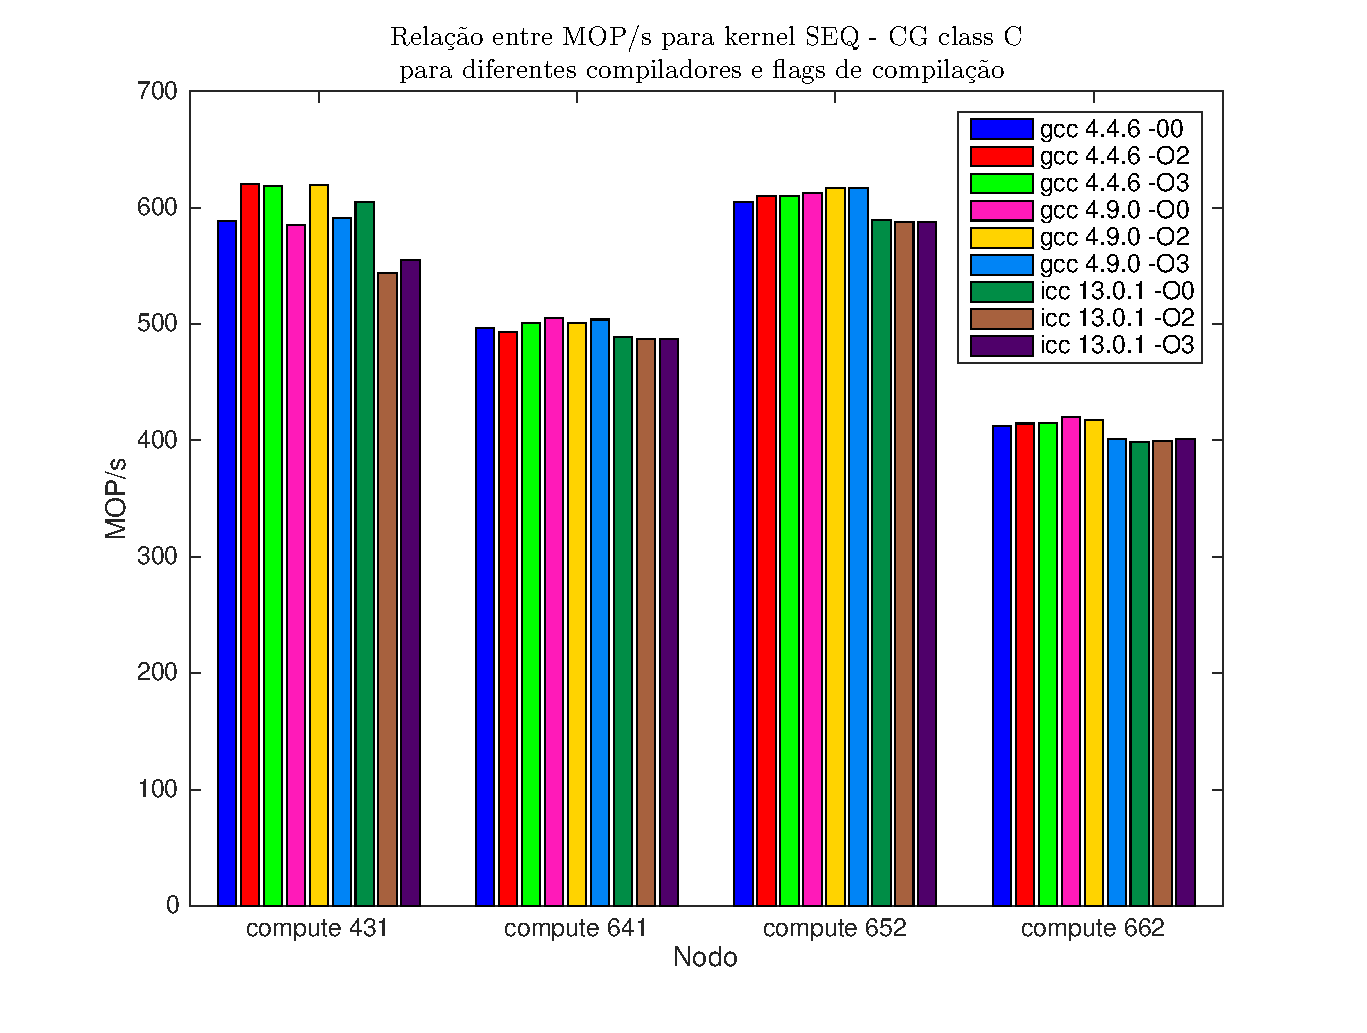
\includegraphics[width=1.1\columnwidth]{EPS/SEQ/MOPS_seq_cg_C.eps}
\caption{Milhões de FP Operations alcançado para o kernel SEQ - CG, classe de dados C para diferentes compiladores e flags de compilação}
\label{mops_seq_cg_c}
\end{figure}

\begin{figure}[H]
\centering
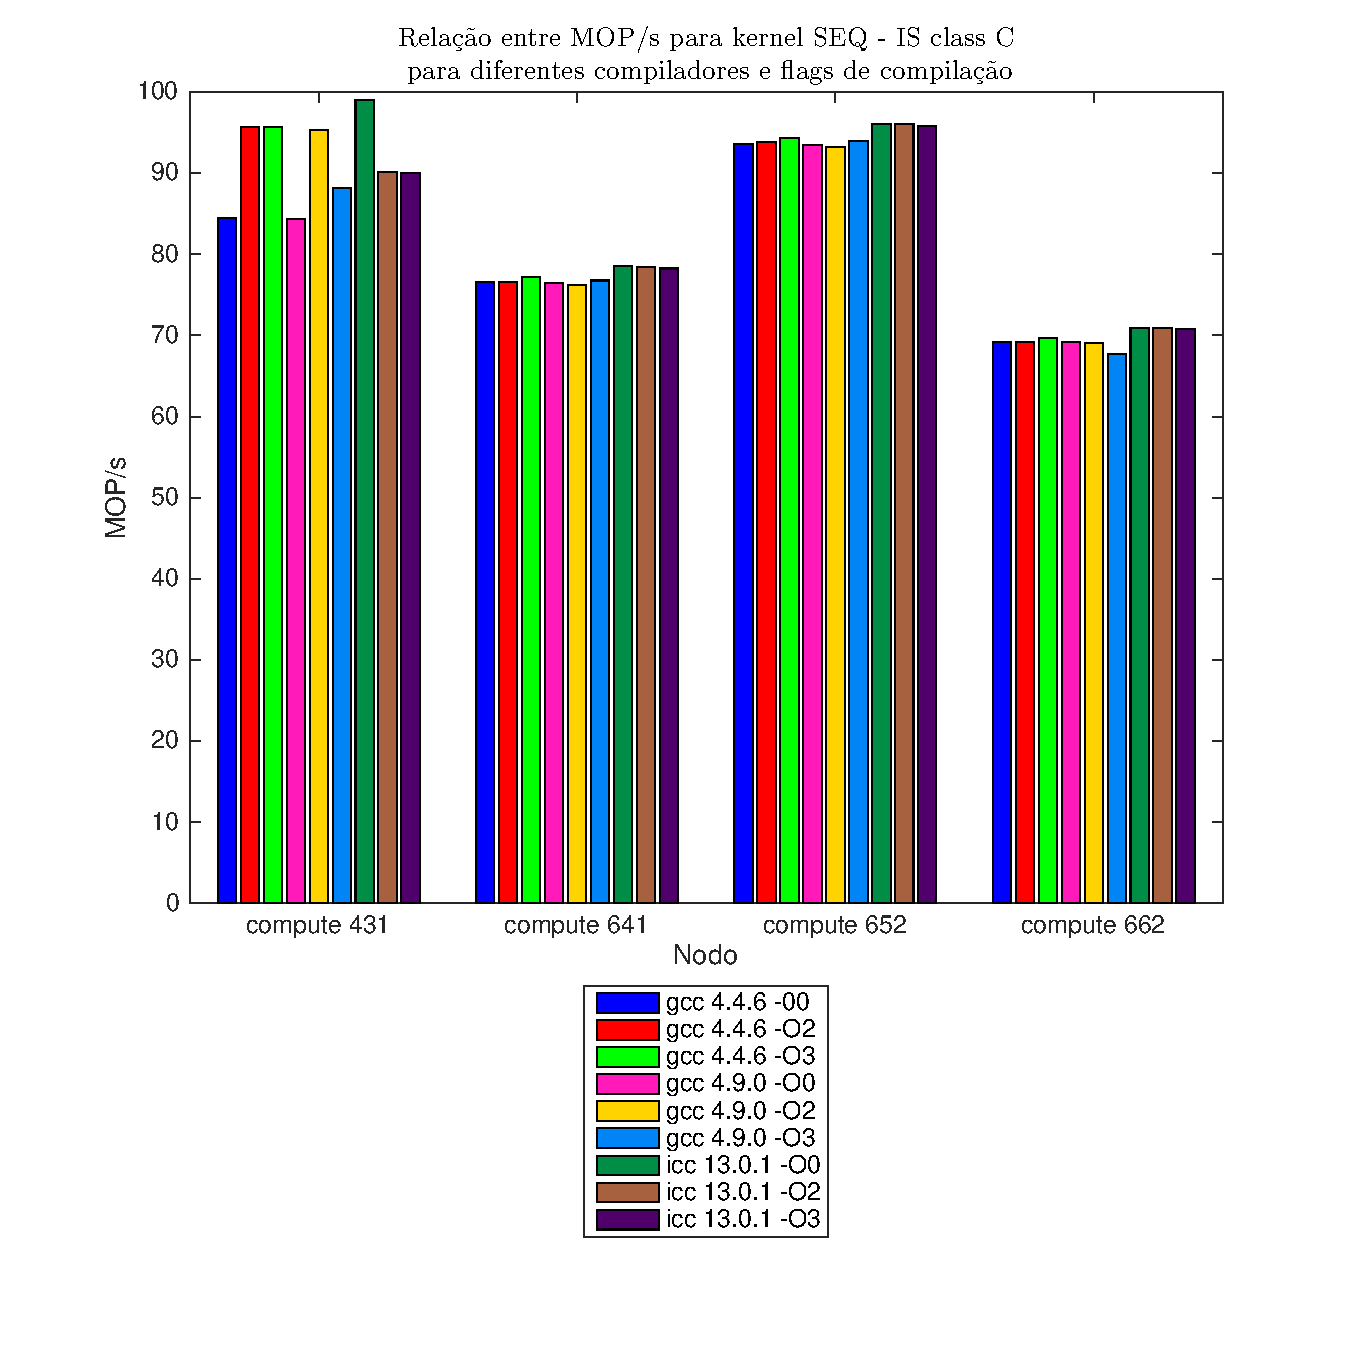
\includegraphics[width=1.1\columnwidth]{EPS/SEQ/MOPS_seq_is_C.eps}
\caption{Milhões de FP Operations alcançado para o kernel SEQ - IS, classe de dados C para diferentes compiladores e flags de compilação}
\label{mops_seq_is_c}
\end{figure}

\begin{figure}[H]
\centering
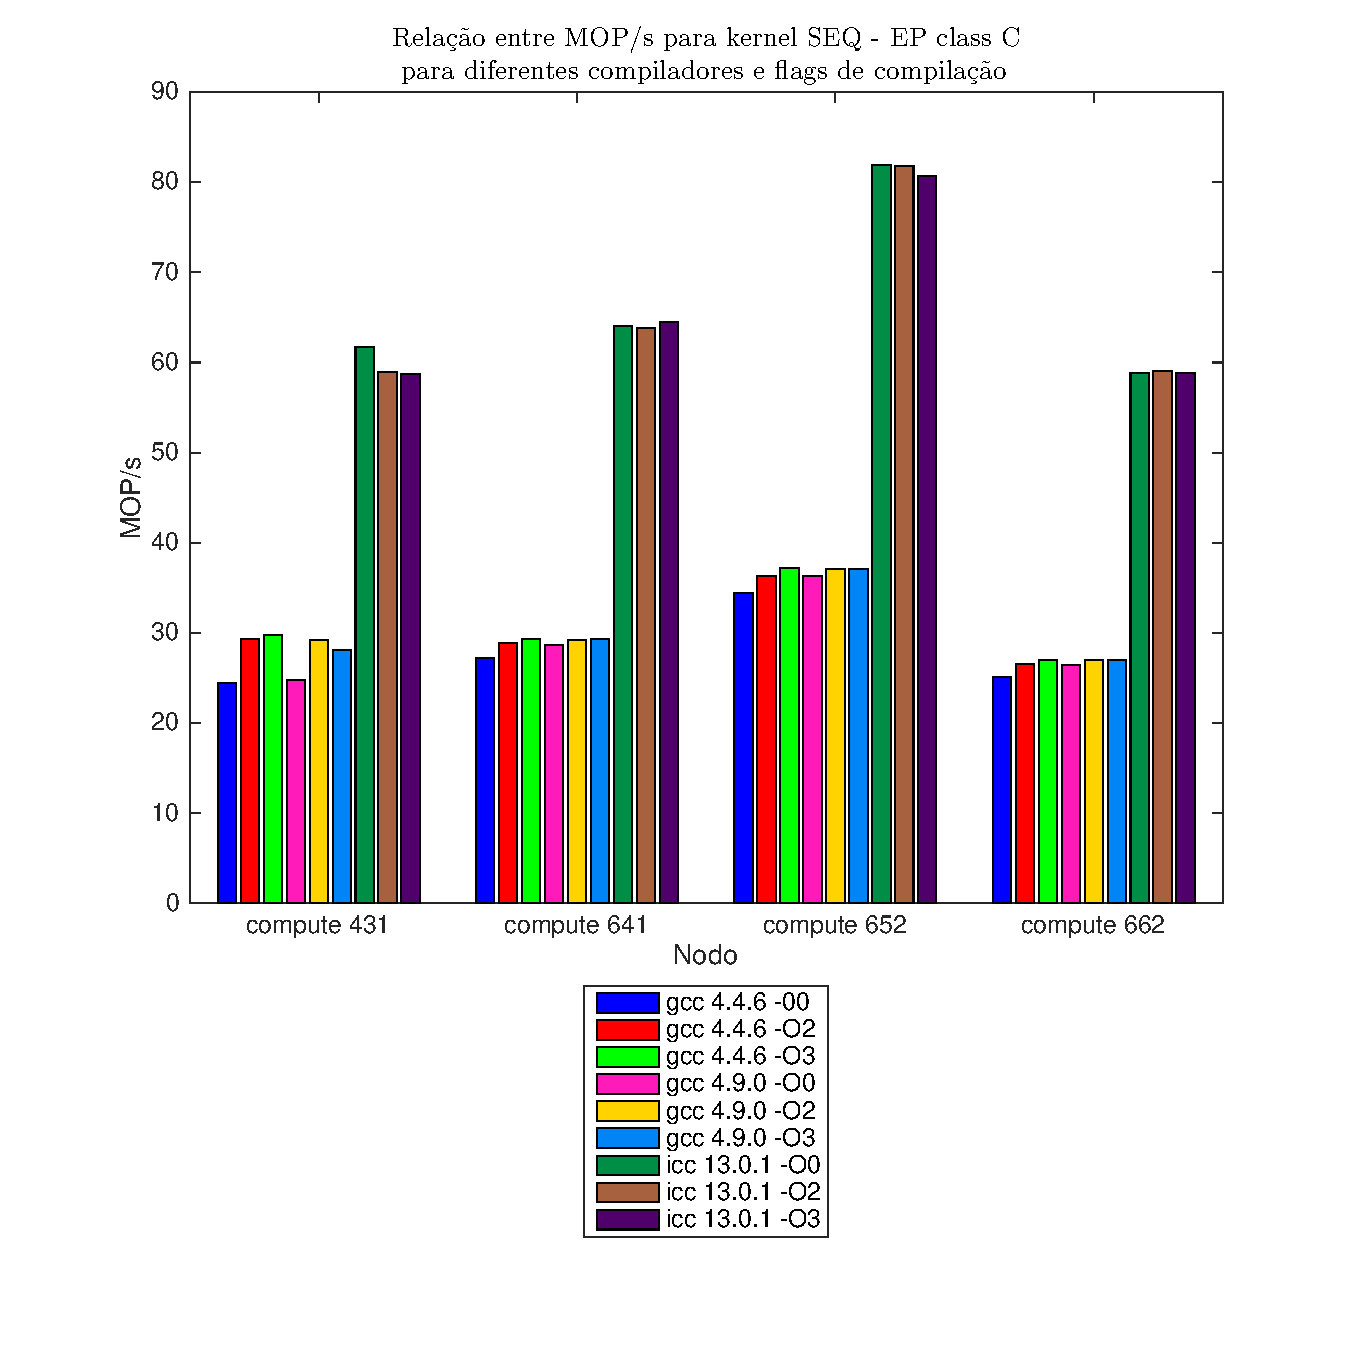
\includegraphics[width=1.1\columnwidth]{EPS/SEQ/MOPS_seq_ep_C.eps}
\caption{Milhões de FP Operations alcançado para o kernel SEQ - EP, classe de dados C para diferentes compiladores e flags de compilação}
\label{mops_seq_ep_c}
\end{figure}

\begin{figure}[H]
\centering
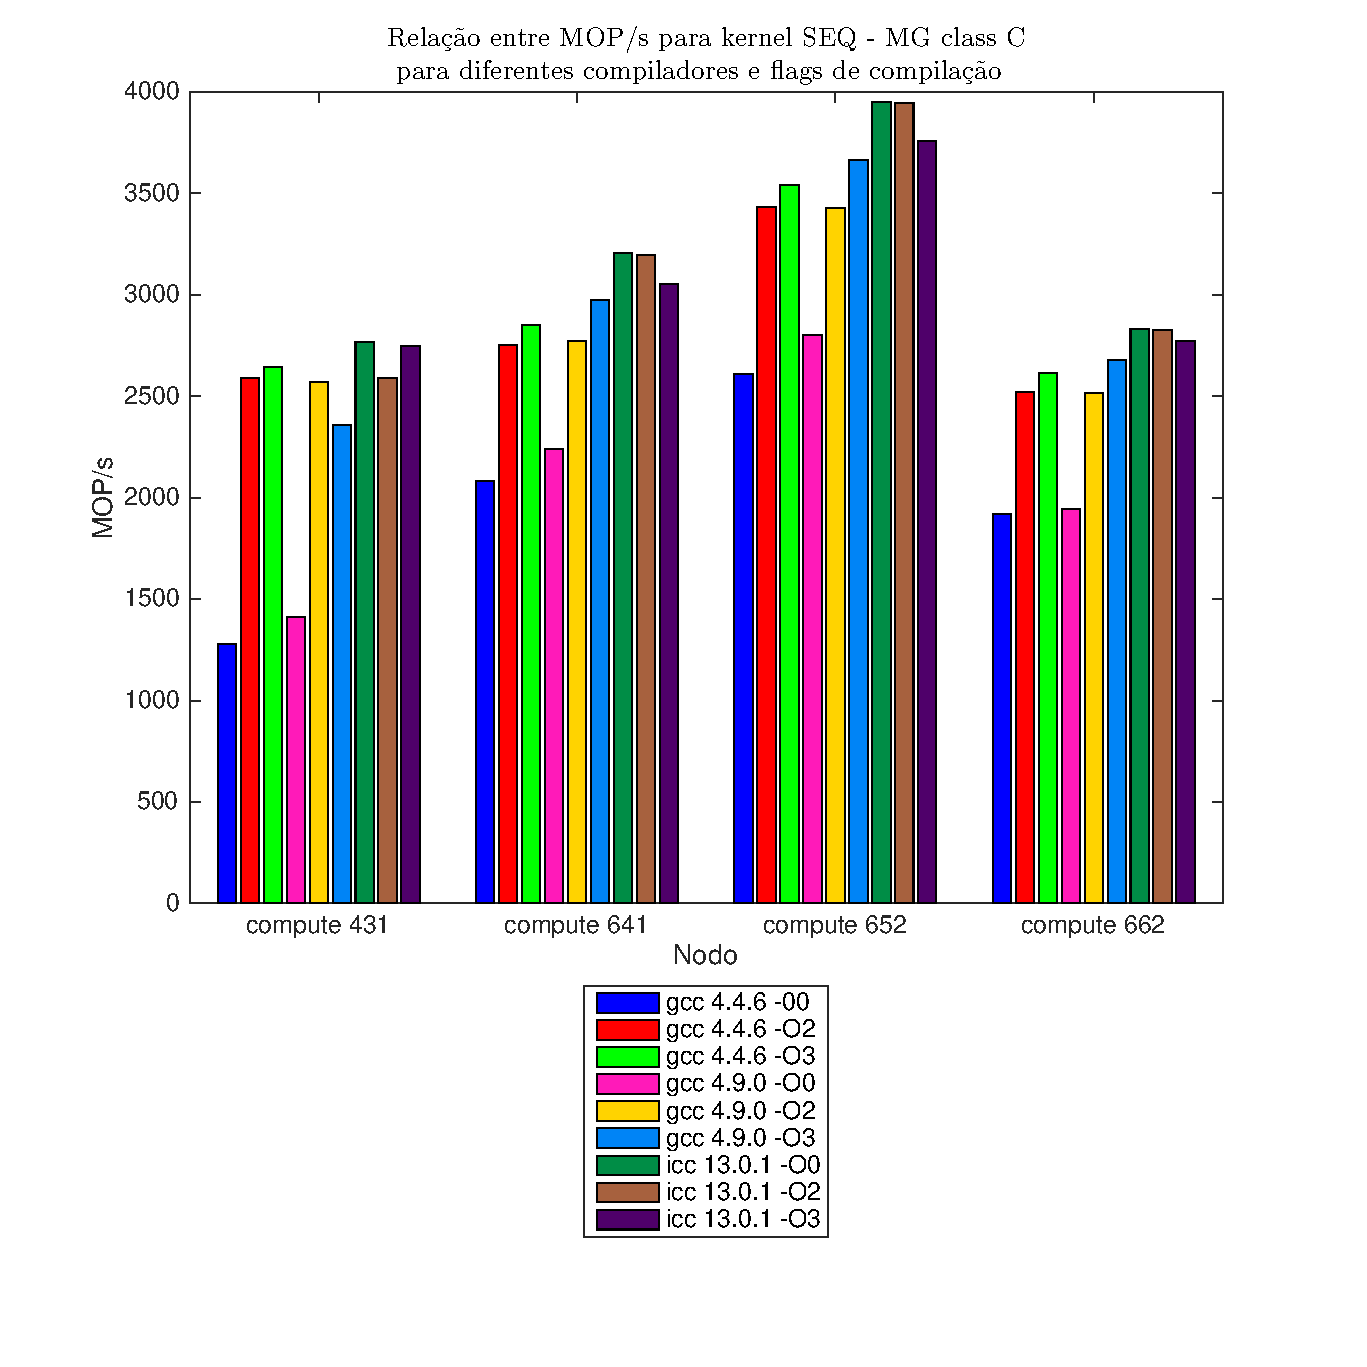
\includegraphics[width=1.1\columnwidth]{EPS/SEQ/MOPS_seq_mg_C.eps}
\caption{Milhões de FP Operations alcançado para o kernel SEQ - MG, classe de dados C para diferentes compiladores e flags de compilação}
\label{mops_seq_mg_c}
\end{figure}


  \end{frame}
  
  


\end{document}




